%%%% ijcai15.tex

\typeout{Automating the Ontological Argument}

% These are the instructions for authors for IJCAI-15.
% They are the same as the ones for IJCAI-11 with superficical wording
%   changes only.

\documentclass{article}
% The file ijcai15.sty is the style file for IJCAI-15 (same as ijcai07.sty).
\usepackage{ijcai15}

% Use the postscript times font!
\usepackage{times}

% the following package is optional:
%\usepackage{latexsym} 

% Following comment is from ijcai97-submit.tex:
% The preparation of these files was supported by Schlumberger Palo Alto
% Research, AT\&T Bell Laboratories, and Morgan Kaufmann Publishers.
% Shirley Jowell, of Morgan Kaufmann Publishers, and Peter F.
% Patel-Schneider, of AT\&T Bell Laboratories collaborated on their
% preparation.

% These instructions can be modified and used in other conferences as long
% as credit to the authors and supporting agencies is retained, this notice
% is not changed, and further modification or reuse is not restricted.
% Neither Shirley Jowell nor Peter F. Patel-Schneider can be listed as
% contacts for providing assistance without their prior permission.

% To use for other conferences, change references to files and the
% conference appropriate and use other authors, contacts, publishers, and
% organizations.
% Also change the deadline and address for returning papers and the length and
% page charge instructions.
% Put where the files are available in the appropriate places.

\usepackage{graphicx}


\title{Automating the Ontological Argument}
\author{Christoph Benzmüller\thanks{German Research Foundation DFG \ldots} and Bruno Woltzenlogel Paleo}
\author{}

\begin{document}

\maketitle

\begin{abstract}
  Higher-order automated theorem provers have revealed some
  philosophically profound new knowledge in metaphysics.
\end{abstract}

\section{Introduction}
G\"{o}del's ontological argument for the existence of God is frequently
presented as a masterpiece argument in metaphysics. A large body of
literature is available which discusses G\"{o}del's original work and/or
subsequent variants of it.

This paper presents an in depth analysis of G\"{o}del's original version
of the ontological argument.   

The analysis has been conducted with automated theorem provers for
classical higher-order logic (HOL). However, since higher-order modal
logic is actually required for the encoding of G\"{o}del's argument, we
utilize an semantic embedding of HOML in HOL.


First applications of theorem proving technology in metaphysics
appeared in 199? in the work Zalta and Oppenheimer.  Further work also
includes Rushby \ldots. Different to what is presented here, none of
these previous formalises and automates variants of HOML, which is
however crucial for G\"{o}del's ontological argument.


The work presented here substantially extends previous work \cite{}.  
The novel contributions of this paper include:

\begin{itemize}
\item Detailed analysis of the inconsistency of G\"{o}del's axioms. The
inconsistency was detected before, but for a long time we were not
able to extract an intuitive argument from the proof of the ATPs.
Further experiments now led to discovery of a surprisingly accessible
understanding of this inconsistency which is philosophically profound
and which has not been presented yet in the respective literature.

\item Fully automated proof of Scott's theorem T3 from the axioms, that
   is, without intermediate argumentation steps as used in previous
   work.

\item Direct verification of modal collapse with Meson in Isabelle/HOL,
which did not work for the previous.

\item On a technical level we show that the novel embedding of S5 is more
    effective than the previous one.

\item Improved syntax presentation.
\end{itemize}

These novel contributions are presented in Sections ? and ?.

In Section ?, novel and previous findings are summarised and discussed 
with regard to their relevance in metaphysics. In this section also 
some further details and improvements on earlier 
findings are presented.

Section ? concludes the paper.



\section{Variants of the Ontological Argument}
Short history, Anselm, Leibniz, etc.
\subsection{G\"{o}del's Proof Script}
\subsection{Scott's Variant}
\subsection{Recent Variants}

\section{Automating HOML in HOL}
\subsection{Outline of the Embedding}
\subsection{Improved Embedding for S5}

\section{Intuitive Inconsistency Argument}
\subsection{LEO-II's Inaccessible Inconsistency Proof}
Tell the story (here or earlier). Show parts of LEO proof.  Inaccessible, but relevant knowledge
is contained.
\begin{figure*}
\centerline{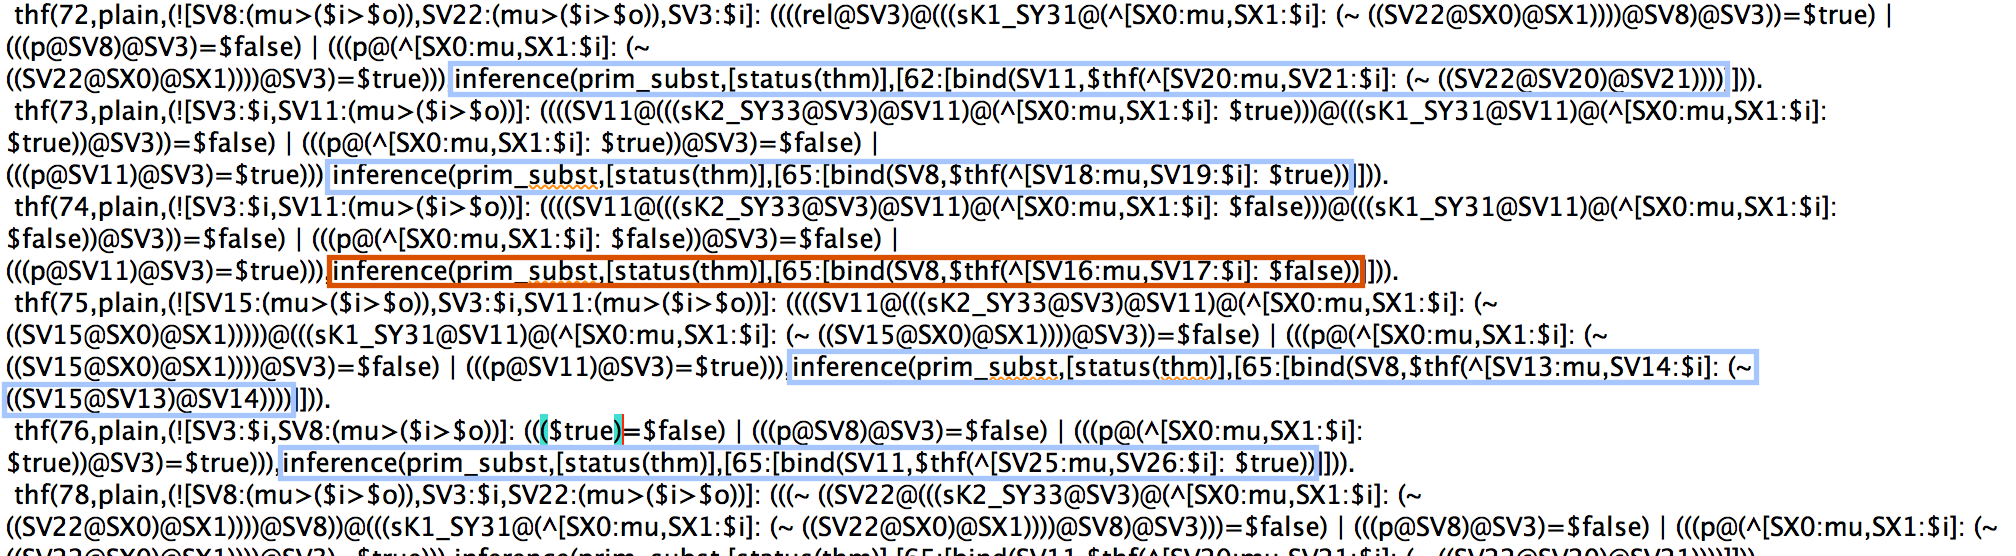
\includegraphics[width=\textwidth]{./Images/LEO-Proof.png}}
\caption{Primitive substitution in LEO-II generates candidates for the
empty property.} \label{LEO-Proof}
\end{figure*}
LEO-II's resolution proof is human unintuitive. However, it contained
relevant hints to the empty property (cf. Fig.~\ref{LEO-Proof}).

\subsection{Argument Reconstruction in Isabelle}
Present the argument informal and in Isabelle (see
Fig.~\ref{InconsistencyIsabelleK}). Easy to understand in 
in KB and KT, slightly harder in K.
\begin{figure}
\centerline{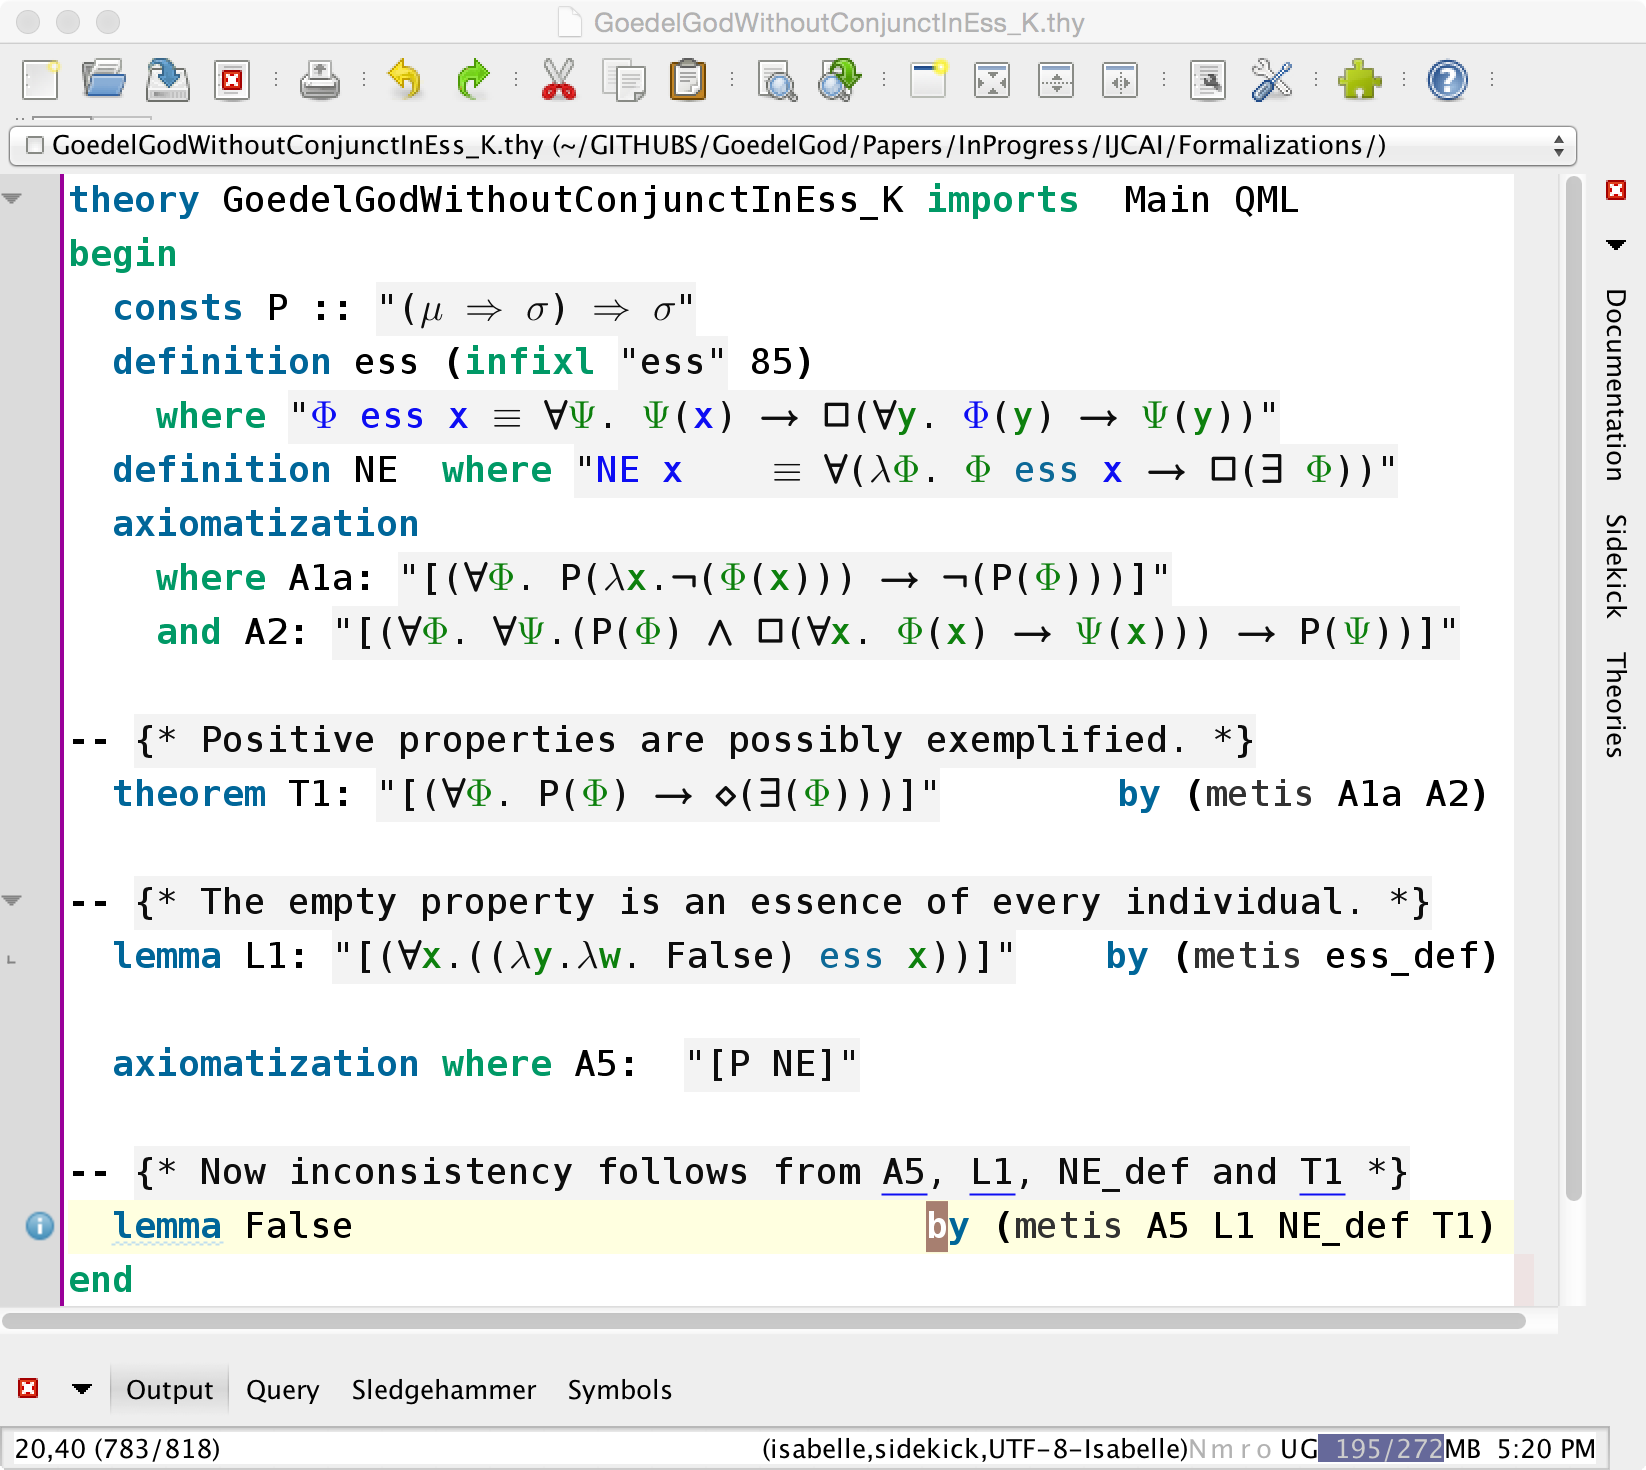
\includegraphics[width=\columnwidth]{./Images/InconsistencyIsabelleK.png}}
\caption{Reconstruction of inconsistency in Isabelle/HOl..} \label{InconsistencyIsabelleK}
\end{figure}


\subsection{Mapping to Gödel's Script}
\begin{figure*}
\centerline{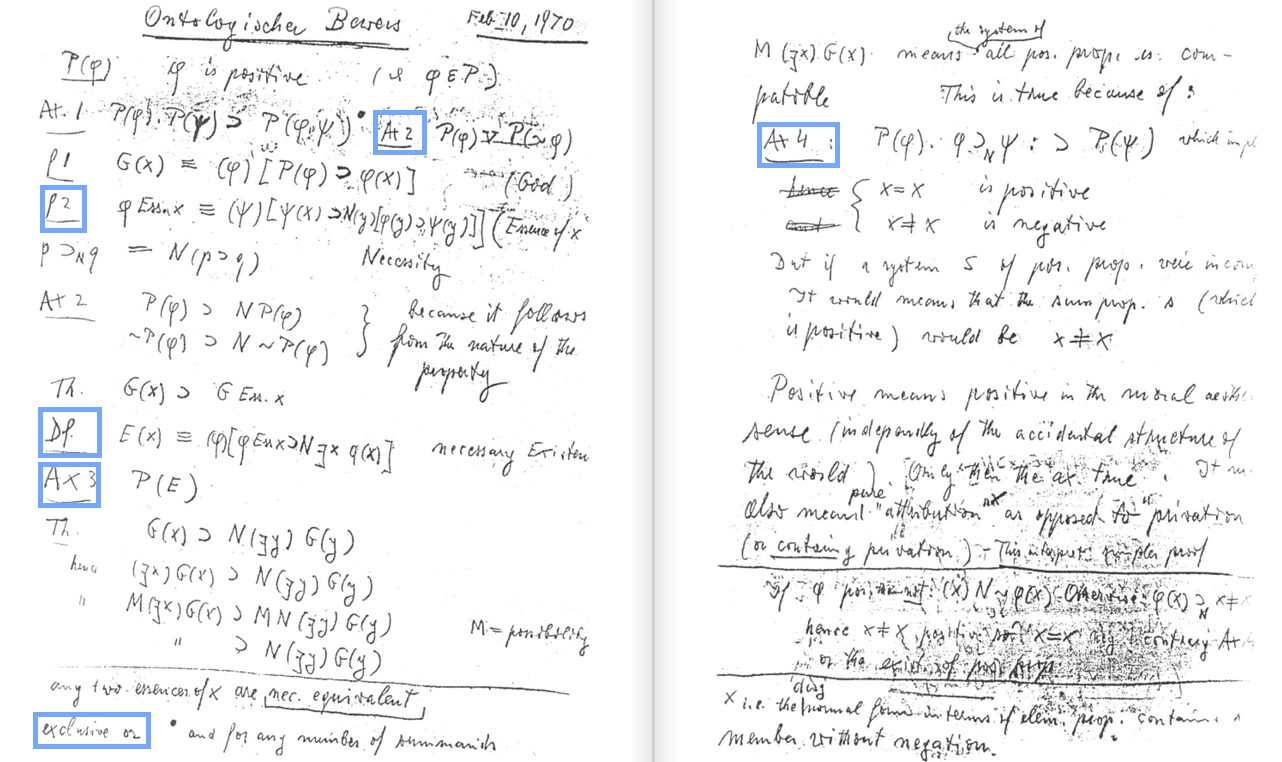
\includegraphics[width=\textwidth]{./Images/Manuscript2.png}}
\caption{Sources of Inconsistence in G\"{o}del's proof script.} \label{GoedelScript}
\end{figure*}

\section{Full Automation of Scott's Proof}
Within the modified logic S5 Scott's proof can be fully automated. The
intermediate argumentation steps as not needed anymore to support the
prover.

In the modified S5 setting also further results can be automatically verified, which 
failed in previous work: verification of  modal collapse in
Isabelle/HOL with Meson.

\section{Conclusion}


Good improvement (technical sense), Sledgehammer can still be improved
(LEO-II finds inconsistency when call directly in THF Syntax, but not
from within Isabelle). Without independent experiments directly in THF 
the inconsistency would thus not have been detected.

\section*{Acknowledgments}

Will be added at a later point.

%German Research Foundation DFG, Chad Brown

\appendix

\section{\LaTeX{} and Word Style Files}\label{stylefiles}

The \LaTeX{} and Word style files are available on the IJCAI--15
website, {\tt http://www.ijcai-15.org/}.
These style files implement the formatting instructions in this
document.

The \LaTeX{} files are {\tt ijcai15.sty} and {\tt ijcai15.tex}, and
the Bib\TeX{} files are {\tt named.bst} and {\tt ijcai15.bib}. The
\LaTeX{} style file is for version 2e of \LaTeX{}, and the Bib\TeX{}
style file is for version 0.99c of Bib\TeX{} ({\em not} version
0.98i). The {\tt ijcai15.sty} file is the same as the {\tt
ijcai07.sty} file used for IJCAI--07.

The Microsoft Word style file consists of a single file, {\tt
ijcai15.doc}. This template is the same as the one used for
IJCAI--07.

These Microsoft Word and \LaTeX{} files contain the source of the
present document and may serve as a formatting sample.  

Further information on using these styles for the preparation of
papers for IJCAI--15 can be obtained by contacting {\tt
pcchair15@ijcai.org}.

%% The file named.bst is a bibliography style file for BibTeX 0.99c
\bibliographystyle{named}
\bibliography{ijcai15}

\end{document}

